\documentclass[1p]{elsarticle_modified}
%\bibliographystyle{elsarticle-num}

%\usepackage[colorlinks]{hyperref}
%\usepackage{abbrmath_seonhwa} %\Abb, \Ascr, \Acal ,\Abf, \Afrak
\usepackage{amsfonts}
\usepackage{amssymb}
\usepackage{amsmath}
\usepackage{amsthm}
\usepackage{scalefnt}
\usepackage{amsbsy}
\usepackage{kotex}
\usepackage{caption}
\usepackage{subfig}
\usepackage{color}
\usepackage{graphicx}
\usepackage{xcolor} %% white, black, red, green, blue, cyan, magenta, yellow
\usepackage{float}
\usepackage{setspace}
\usepackage{hyperref}

\usepackage{tikz}
\usetikzlibrary{arrows}

\usepackage{multirow}
\usepackage{array} % fixed length table
\usepackage{hhline}

%%%%%%%%%%%%%%%%%%%%%
\makeatletter
\renewcommand*\env@matrix[1][\arraystretch]{%
	\edef\arraystretch{#1}%
	\hskip -\arraycolsep
	\let\@ifnextchar\new@ifnextchar
	\array{*\c@MaxMatrixCols c}}
\makeatother %https://tex.stackexchange.com/questions/14071/how-can-i-increase-the-line-spacing-in-a-matrix
%%%%%%%%%%%%%%%

\usepackage[normalem]{ulem}

\newcommand{\msout}[1]{\ifmmode\text{\sout{\ensuremath{#1}}}\else\sout{#1}\fi}
%SOURCE: \msout is \stkout macro in https://tex.stackexchange.com/questions/20609/strikeout-in-math-mode

\newcommand{\cancel}[1]{
	\ifmmode
	{\color{red}\msout{#1}}
	\else
	{\color{red}\sout{#1}}
	\fi
}

\newcommand{\add}[1]{
	{\color{blue}\uwave{#1}}
}

\newcommand{\replace}[2]{
	\ifmmode
	{\color{red}\msout{#1}}{\color{blue}\uwave{#2}}
	\else
	{\color{red}\sout{#1}}{\color{blue}\uwave{#2}}
	\fi
}

\newcommand{\Sol}{\mathcal{S}} %segment
\newcommand{\D}{D} %diagram
\newcommand{\A}{\mathcal{A}} %arc


%%%%%%%%%%%%%%%%%%%%%%%%%%%%%5 test

\def\sl{\operatorname{\textup{SL}}(2,\Cbb)}
\def\psl{\operatorname{\textup{PSL}}(2,\Cbb)}
\def\quan{\mkern 1mu \triangleright \mkern 1mu}

\theoremstyle{definition}
\newtheorem{thm}{Theorem}[section]
\newtheorem{prop}[thm]{Proposition}
\newtheorem{lem}[thm]{Lemma}
\newtheorem{ques}[thm]{Question}
\newtheorem{cor}[thm]{Corollary}
\newtheorem{defn}[thm]{Definition}
\newtheorem{exam}[thm]{Example}
\newtheorem{rmk}[thm]{Remark}
\newtheorem{alg}[thm]{Algorithm}

\newcommand{\I}{\sqrt{-1}}
\begin{document}

%\begin{frontmatter}
%
%\title{Boundary parabolic representations of knots up to 8 crossings}
%
%%% Group authors per affiliation:
%\author{Yunhi Cho} 
%\address{Department of Mathematics, University of Seoul, Seoul, Korea}
%\ead{yhcho@uos.ac.kr}
%
%
%\author{Seonhwa Kim} %\fnref{s_kim}}
%\address{Center for Geometry and Physics, Institute for Basic Science, Pohang, 37673, Korea}
%\ead{ryeona17@ibs.re.kr}
%
%\author{Hyuk Kim}
%\address{Department of Mathematical Sciences, Seoul National University, Seoul 08826, Korea}
%\ead{hyukkim@snu.ac.kr}
%
%\author{Seokbeom Yoon}
%\address{Department of Mathematical Sciences, Seoul National University, Seoul, 08826,  Korea}
%\ead{sbyoon15@snu.ac.kr}
%
%\begin{abstract}
%We find all boundary parabolic representation of knots up to 8 crossings.
%
%\end{abstract}
%\begin{keyword}
%    \MSC[2010] 57M25 
%\end{keyword}
%
%\end{frontmatter}

%\linenumbers
%\tableofcontents
%
\newcommand\colored[1]{\textcolor{white}{\rule[-0.35ex]{0.8em}{1.4ex}}\kern-0.8em\color{red} #1}%
%\newcommand\colored[1]{\textcolor{white}{ #1}\kern-2.17ex	\textcolor{white}{ #1}\kern-1.81ex	\textcolor{white}{ #1}\kern-2.15ex\color{red}#1	}

{\Large $\underline{12n_{0787}~(K12n_{0787})}$}

\setlength{\tabcolsep}{10pt}
\renewcommand{\arraystretch}{1.6}
\vspace{1cm}\begin{tabular}{m{100pt}>{\centering\arraybackslash}m{274pt}}
\multirow{5}{120pt}{
	\centering
	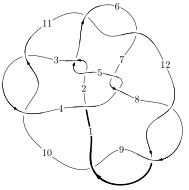
\includegraphics[width=112pt]{../../../GIT/diagram.site/Diagrams/png/2876_12n_0787.png}\\
\ \ \ A knot diagram\footnotemark}&
\allowdisplaybreaks
\textbf{Linearized knot diagam} \\
\cline{2-2}
 &
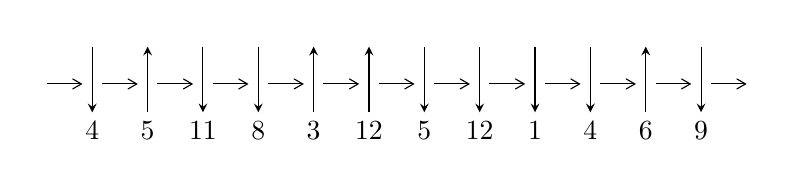
\begin{tikzpicture}[x=20pt, y=17pt]
	% nodes
	\node (C0) at (0, 0) {};
	\node (C1) at (1, 0) {};
	\node (C1U) at (1, +1) {};
	\node (C1D) at (1, -1) {4};

	\node (C2) at (2, 0) {};
	\node (C2U) at (2, +1) {};
	\node (C2D) at (2, -1) {5};

	\node (C3) at (3, 0) {};
	\node (C3U) at (3, +1) {};
	\node (C3D) at (3, -1) {11};

	\node (C4) at (4, 0) {};
	\node (C4U) at (4, +1) {};
	\node (C4D) at (4, -1) {8};

	\node (C5) at (5, 0) {};
	\node (C5U) at (5, +1) {};
	\node (C5D) at (5, -1) {3};

	\node (C6) at (6, 0) {};
	\node (C6U) at (6, +1) {};
	\node (C6D) at (6, -1) {12};

	\node (C7) at (7, 0) {};
	\node (C7U) at (7, +1) {};
	\node (C7D) at (7, -1) {5};

	\node (C8) at (8, 0) {};
	\node (C8U) at (8, +1) {};
	\node (C8D) at (8, -1) {12};

	\node (C9) at (9, 0) {};
	\node (C9U) at (9, +1) {};
	\node (C9D) at (9, -1) {1};

	\node (C10) at (10, 0) {};
	\node (C10U) at (10, +1) {};
	\node (C10D) at (10, -1) {4};

	\node (C11) at (11, 0) {};
	\node (C11U) at (11, +1) {};
	\node (C11D) at (11, -1) {6};

	\node (C12) at (12, 0) {};
	\node (C12U) at (12, +1) {};
	\node (C12D) at (12, -1) {9};
	\node (C13) at (13, 0) {};

	% arrows
	\draw[->,>={angle 60}]
	(C0) edge (C1) (C1) edge (C2) (C2) edge (C3) (C3) edge (C4) (C4) edge (C5) (C5) edge (C6) (C6) edge (C7) (C7) edge (C8) (C8) edge (C9) (C9) edge (C10) (C10) edge (C11) (C11) edge (C12) (C12) edge (C13) ;	\draw[->,>=stealth]
	(C1U) edge (C1D) (C2D) edge (C2U) (C3U) edge (C3D) (C4U) edge (C4D) (C5D) edge (C5U) (C6D) edge (C6U) (C7U) edge (C7D) (C8U) edge (C8D) (C9U) edge (C9D) (C10U) edge (C10D) (C11D) edge (C11U) (C12U) edge (C12D) ;
	\end{tikzpicture} \\
\hhline{~~} \\& 
\textbf{Solving Sequence} \\ \cline{2-2} 
 &
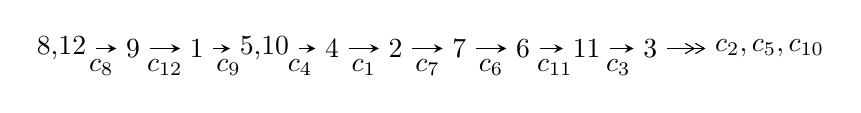
\begin{tikzpicture}[x=23pt, y=7pt]
	% node
	\node (A0) at (-1/8, 0) {8,12};
	\node (A1) at (1, 0) {9};
	\node (A2) at (2, 0) {1};
	\node (A3) at (49/16, 0) {5,10};
	\node (A4) at (33/8, 0) {4};
	\node (A5) at (41/8, 0) {2};
	\node (A6) at (49/8, 0) {7};
	\node (A7) at (57/8, 0) {6};
	\node (A8) at (65/8, 0) {11};
	\node (A9) at (73/8, 0) {3};
	\node (C1) at (1/2, -1) {$c_{8}$};
	\node (C2) at (3/2, -1) {$c_{12}$};
	\node (C3) at (5/2, -1) {$c_{9}$};
	\node (C4) at (29/8, -1) {$c_{4}$};
	\node (C5) at (37/8, -1) {$c_{1}$};
	\node (C6) at (45/8, -1) {$c_{7}$};
	\node (C7) at (53/8, -1) {$c_{6}$};
	\node (C8) at (61/8, -1) {$c_{11}$};
	\node (C9) at (69/8, -1) {$c_{3}$};
	\node (A10) at (11, 0) {$c_{2},c_{5},c_{10}$};

	% edge
	\draw[->,>=stealth]	
	(A0) edge (A1) (A1) edge (A2) (A2) edge (A3) (A3) edge (A4) (A4) edge (A5) (A5) edge (A6) (A6) edge (A7) (A7) edge (A8) (A8) edge (A9) ;
	\draw[->>,>={angle 60}]	
	(A9) edge (A10);
\end{tikzpicture} \\ 

\end{tabular} \\

\footnotetext{
The image of knot diagram is generated by the software ``\textbf{Draw programme}" developed by Andrew Bartholomew(\url{http://www.layer8.co.uk/maths/draw/index.htm\#Running-draw}), where we modified some parts for our purpose(\url{https://github.com/CATsTAILs/LinksPainter}).
}\phantom \\ \newline 
\centering \textbf{Ideals for irreducible components\footnotemark of $X_{\text{par}}$} 
 
\begin{align*}
I^u_{1}&=\langle 
-4.86056\times10^{58} u^{51}-6.69927\times10^{58} u^{50}+\cdots+6.23296\times10^{59} b+8.49108\times10^{59},\\
\phantom{I^u_{1}}&\phantom{= \langle  }-6.68649\times10^{58} u^{51}+2.75220\times10^{59} u^{50}+\cdots+4.79459\times10^{58} a+8.71827\times10^{59},\\
\phantom{I^u_{1}}&\phantom{= \langle  }u^{52}-4 u^{51}+\cdots+18 u+1\rangle \\
I^u_{2}&=\langle 
- u^{16}- u^{15}+\cdots+b+1,\;2 u^{16}+u^{15}+\cdots+a-6 u,\;u^{17}+u^{16}+\cdots-2 u-1\rangle \\
\\
\end{align*}
\raggedright * 2 irreducible components of $\dim_{\mathbb{C}}=0$, with total 69 representations.\\
\footnotetext{All coefficients of polynomials are rational numbers. But the coefficients are sometimes approximated in decimal forms when there is not enough margin.}
\newpage
\renewcommand{\arraystretch}{1}
\centering \section*{I. $I^u_{1}= \langle -4.86\times10^{58} u^{51}-6.70\times10^{58} u^{50}+\cdots+6.23\times10^{59} b+8.49\times10^{59},\;-6.69\times10^{58} u^{51}+2.75\times10^{59} u^{50}+\cdots+4.79\times10^{58} a+8.72\times10^{59},\;u^{52}-4 u^{51}+\cdots+18 u+1 \rangle$}
\flushleft \textbf{(i) Arc colorings}\\
\begin{tabular}{m{7pt} m{180pt} m{7pt} m{180pt} }
\flushright $a_{8}=$&$\begin{pmatrix}1\\0\end{pmatrix}$ \\
\flushright $a_{12}=$&$\begin{pmatrix}0\\u\end{pmatrix}$ \\
\flushright $a_{9}=$&$\begin{pmatrix}1\\u^2\end{pmatrix}$ \\
\flushright $a_{1}=$&$\begin{pmatrix}- u\\- u^3+u\end{pmatrix}$ \\
\flushright $a_{5}=$&$\begin{pmatrix}1.39459 u^{51}-5.74023 u^{50}+\cdots+155.294 u-18.1836\\0.0779815 u^{51}+0.107481 u^{50}+\cdots-22.1919 u-1.36229\end{pmatrix}$ \\
\flushright $a_{10}=$&$\begin{pmatrix}- u^2+1\\- u^4+2 u^2\end{pmatrix}$ \\
\flushright $a_{4}=$&$\begin{pmatrix}1.47257 u^{51}-5.63275 u^{50}+\cdots+133.102 u-19.5459\\0.0779815 u^{51}+0.107481 u^{50}+\cdots-22.1919 u-1.36229\end{pmatrix}$ \\
\flushright $a_{2}=$&$\begin{pmatrix}-4.28758 u^{51}+17.1080 u^{50}+\cdots-1091.27 u-36.3160\\0.0338379 u^{51}-0.0711693 u^{50}+\cdots-2.55862 u+1.27029\end{pmatrix}$ \\
\flushright $a_{7}=$&$\begin{pmatrix}-1.21648 u^{51}+4.74618 u^{50}+\cdots-367.518 u-25.5631\\-0.0685253 u^{51}+0.296845 u^{50}+\cdots-8.41934 u+0.118102\end{pmatrix}$ \\
\flushright $a_{6}=$&$\begin{pmatrix}-1.21648 u^{51}+4.74618 u^{50}+\cdots-367.518 u-25.5631\\-0.194638 u^{51}+0.560317 u^{50}+\cdots-5.04742 u+0.237849\end{pmatrix}$ \\
\flushright $a_{11}=$&$\begin{pmatrix}1.55761 u^{51}-6.02658 u^{50}+\cdots+450.253 u+35.6977\\0.0494698 u^{51}-0.154809 u^{50}+\cdots+12.1116 u-0.0549377\end{pmatrix}$ \\
\flushright $a_{3}=$&$\begin{pmatrix}-1.21792 u^{51}+5.14238 u^{50}+\cdots-481.653 u-35.7438\\-0.124343 u^{51}+0.226786 u^{50}+\cdots-5.42725 u+0.405315\end{pmatrix}$\\&\end{tabular}
\flushleft \textbf{(ii) Obstruction class $= -1$}\\~\\
\flushleft \textbf{(iii) Cusp Shapes $= 0.948355 u^{51}-2.66963 u^{50}+\cdots+228.868 u+10.1763$}\\~\\
\newpage\renewcommand{\arraystretch}{1}
\flushleft \textbf{(iv) u-Polynomials at the component}\newline \\
\begin{tabular}{m{50pt}|m{274pt}}
Crossings & \hspace{64pt}u-Polynomials at each crossing \\
\hline $$\begin{aligned}c_{1}\end{aligned}$$&$\begin{aligned}
&u^{52}-9 u^{51}+\cdots+27964 u-1601
\end{aligned}$\\
\hline $$\begin{aligned}c_{2},c_{5}\end{aligned}$$&$\begin{aligned}
&u^{52}-2 u^{51}+\cdots+273 u+131
\end{aligned}$\\
\hline $$\begin{aligned}c_{3},c_{10}\end{aligned}$$&$\begin{aligned}
&u^{52}- u^{51}+\cdots+455 u+47
\end{aligned}$\\
\hline $$\begin{aligned}c_{4},c_{7}\end{aligned}$$&$\begin{aligned}
&u^{52}-3 u^{51}+\cdots+6 u-1
\end{aligned}$\\
\hline $$\begin{aligned}c_{6},c_{11}\end{aligned}$$&$\begin{aligned}
&u^{52}-14 u^{50}+\cdots-1895 u+425
\end{aligned}$\\
\hline $$\begin{aligned}c_{8},c_{9},c_{12}\end{aligned}$$&$\begin{aligned}
&u^{52}+4 u^{51}+\cdots-18 u+1
\end{aligned}$\\
\hline
\end{tabular}\\~\\
\newpage\renewcommand{\arraystretch}{1}
\flushleft \textbf{(v) Riley Polynomials at the component}\newline \\
\begin{tabular}{m{50pt}|m{274pt}}
Crossings & \hspace{64pt}Riley Polynomials at each crossing \\
\hline $$\begin{aligned}c_{1}\end{aligned}$$&$\begin{aligned}
&y^{52}-69 y^{51}+\cdots+3606192 y+2563201
\end{aligned}$\\
\hline $$\begin{aligned}c_{2},c_{5}\end{aligned}$$&$\begin{aligned}
&y^{52}-26 y^{51}+\cdots-263693 y+17161
\end{aligned}$\\
\hline $$\begin{aligned}c_{3},c_{10}\end{aligned}$$&$\begin{aligned}
&y^{52}+19 y^{51}+\cdots-52301 y+2209
\end{aligned}$\\
\hline $$\begin{aligned}c_{4},c_{7}\end{aligned}$$&$\begin{aligned}
&y^{52}+13 y^{51}+\cdots-80 y+1
\end{aligned}$\\
\hline $$\begin{aligned}c_{6},c_{11}\end{aligned}$$&$\begin{aligned}
&y^{52}-28 y^{51}+\cdots-3054675 y+180625
\end{aligned}$\\
\hline $$\begin{aligned}c_{8},c_{9},c_{12}\end{aligned}$$&$\begin{aligned}
&y^{52}-68 y^{51}+\cdots+260 y+1
\end{aligned}$\\
\hline
\end{tabular}\\~\\
\newpage\flushleft \textbf{(vi) Complex Volumes and Cusp Shapes}
$$\begin{array}{c|c|c}  
\text{Solutions to }I^u_{1}& \I (\text{vol} + \sqrt{-1}CS) & \text{Cusp shape}\\
 \hline 
\begin{aligned}
u &= -0.963102 + 0.345038 I \\
a &= \phantom{-}0.367913 + 0.884454 I \\
b &= -0.701674 - 0.540338 I\end{aligned}
 & \phantom{-}1.19699 + 4.57480 I & \phantom{-0.000000 } 0 \\ \hline\begin{aligned}
u &= -0.963102 - 0.345038 I \\
a &= \phantom{-}0.367913 - 0.884454 I \\
b &= -0.701674 + 0.540338 I\end{aligned}
 & \phantom{-}1.19699 - 4.57480 I & \phantom{-0.000000 } 0 \\ \hline\begin{aligned}
u &= \phantom{-}1.010440 + 0.226511 I \\
a &= -0.195406 + 0.336697 I \\
b &= -0.565644 - 0.187214 I\end{aligned}
 & -1.74134 - 0.12755 I & \phantom{-0.000000 } 0 \\ \hline\begin{aligned}
u &= \phantom{-}1.010440 - 0.226511 I \\
a &= -0.195406 - 0.336697 I \\
b &= -0.565644 + 0.187214 I\end{aligned}
 & -1.74134 + 0.12755 I & \phantom{-0.000000 } 0 \\ \hline\begin{aligned}
u &= -0.284882 + 1.011440 I \\
a &= \phantom{-}0.769715 + 0.747090 I \\
b &= -0.604356 - 0.603378 I\end{aligned}
 & \phantom{-}3.70336 - 4.26964 I & \phantom{-0.000000 } 0 \\ \hline\begin{aligned}
u &= -0.284882 - 1.011440 I \\
a &= \phantom{-}0.769715 - 0.747090 I \\
b &= -0.604356 + 0.603378 I\end{aligned}
 & \phantom{-}3.70336 + 4.26964 I & \phantom{-0.000000 } 0 \\ \hline\begin{aligned}
u &= -0.654100 + 0.538210 I \\
a &= \phantom{-}0.26052 + 1.52753 I \\
b &= \phantom{-}0.855051 - 0.775108 I\end{aligned}
 & -1.64856 + 4.08097 I & -3.59358 - 7.53580 I \\ \hline\begin{aligned}
u &= -0.654100 - 0.538210 I \\
a &= \phantom{-}0.26052 - 1.52753 I \\
b &= \phantom{-}0.855051 + 0.775108 I\end{aligned}
 & -1.64856 - 4.08097 I & -3.59358 + 7.53580 I \\ \hline\begin{aligned}
u &= \phantom{-}1.109320 + 0.362480 I \\
a &= -0.49904 + 1.54272 I \\
b &= -0.519449 - 0.934936 I\end{aligned}
 & \phantom{-}0.59353 - 3.33817 I & \phantom{-0.000000 } 0 \\ \hline\begin{aligned}
u &= \phantom{-}1.109320 - 0.362480 I \\
a &= -0.49904 - 1.54272 I \\
b &= -0.519449 + 0.934936 I\end{aligned}
 & \phantom{-}0.59353 + 3.33817 I & \phantom{-0.000000 } 0\\
 \hline 
 \end{array}$$\newpage$$\begin{array}{c|c|c}  
\text{Solutions to }I^u_{1}& \I (\text{vol} + \sqrt{-1}CS) & \text{Cusp shape}\\
 \hline 
\begin{aligned}
u &= -0.822872 + 0.103062 I \\
a &= \phantom{-}0.257461 + 0.646673 I \\
b &= -0.242471 + 1.056410 I\end{aligned}
 & \phantom{-}6.24954 - 0.94391 I & \phantom{-}0.647108 - 0.326933 I \\ \hline\begin{aligned}
u &= -0.822872 - 0.103062 I \\
a &= \phantom{-}0.257461 - 0.646673 I \\
b &= -0.242471 - 1.056410 I\end{aligned}
 & \phantom{-}6.24954 + 0.94391 I & \phantom{-}0.647108 + 0.326933 I \\ \hline\begin{aligned}
u &= -0.862860 + 0.795004 I \\
a &= \phantom{-}0.01742 - 1.46293 I \\
b &= -0.818392 + 0.955221 I\end{aligned}
 & \phantom{-}1.92110 + 10.19650 I & \phantom{-0.000000 } 0 \\ \hline\begin{aligned}
u &= -0.862860 - 0.795004 I \\
a &= \phantom{-}0.01742 + 1.46293 I \\
b &= -0.818392 - 0.955221 I\end{aligned}
 & \phantom{-}1.92110 - 10.19650 I & \phantom{-0.000000 } 0 \\ \hline\begin{aligned}
u &= \phantom{-}0.940755 + 0.772008 I \\
a &= -0.376983 - 0.720478 I \\
b &= \phantom{-}0.668255 + 0.424349 I\end{aligned}
 & -0.98442 - 3.07513 I & \phantom{-0.000000 } 0 \\ \hline\begin{aligned}
u &= \phantom{-}0.940755 - 0.772008 I \\
a &= -0.376983 + 0.720478 I \\
b &= \phantom{-}0.668255 - 0.424349 I\end{aligned}
 & -0.98442 + 3.07513 I & \phantom{-0.000000 } 0 \\ \hline\begin{aligned}
u &= -0.038382 + 0.763918 I \\
a &= \phantom{-}0.34582 - 2.02691 I \\
b &= -0.418556 + 0.708156 I\end{aligned}
 & \phantom{-}4.27045 - 0.69241 I & \phantom{-}2.11238 - 0.92531 I \\ \hline\begin{aligned}
u &= -0.038382 - 0.763918 I \\
a &= \phantom{-}0.34582 + 2.02691 I \\
b &= -0.418556 - 0.708156 I\end{aligned}
 & \phantom{-}4.27045 + 0.69241 I & \phantom{-}2.11238 + 0.92531 I \\ \hline\begin{aligned}
u &= \phantom{-}1.251610 + 0.050476 I \\
a &= -0.50166 + 1.68503 I \\
b &= -0.371536 - 1.046800 I\end{aligned}
 & \phantom{-}0.92724 - 3.35039 I & \phantom{-0.000000 } 0 \\ \hline\begin{aligned}
u &= \phantom{-}1.251610 - 0.050476 I \\
a &= -0.50166 - 1.68503 I \\
b &= -0.371536 + 1.046800 I\end{aligned}
 & \phantom{-}0.92724 + 3.35039 I & \phantom{-0.000000 } 0\\
 \hline 
 \end{array}$$\newpage$$\begin{array}{c|c|c}  
\text{Solutions to }I^u_{1}& \I (\text{vol} + \sqrt{-1}CS) & \text{Cusp shape}\\
 \hline 
\begin{aligned}
u &= -1.272460 + 0.135660 I \\
a &= \phantom{-}0.48984 + 1.43474 I \\
b &= -0.144334 - 0.106513 I\end{aligned}
 & \phantom{-}1.17738 + 4.15170 I & \phantom{-0.000000 } 0 \\ \hline\begin{aligned}
u &= -1.272460 - 0.135660 I \\
a &= \phantom{-}0.48984 - 1.43474 I \\
b &= -0.144334 + 0.106513 I\end{aligned}
 & \phantom{-}1.17738 - 4.15170 I & \phantom{-0.000000 } 0 \\ \hline\begin{aligned}
u &= -0.687341 + 0.187968 I \\
a &= -0.167504 - 0.552195 I \\
b &= \phantom{-}0.675651 + 0.912887 I\end{aligned}
 & -1.04394 - 1.60688 I & -0.66527 - 4.34427 I \\ \hline\begin{aligned}
u &= -0.687341 - 0.187968 I \\
a &= -0.167504 + 0.552195 I \\
b &= \phantom{-}0.675651 - 0.912887 I\end{aligned}
 & -1.04394 + 1.60688 I & -0.66527 + 4.34427 I \\ \hline\begin{aligned}
u &= \phantom{-}0.647636 + 0.201060 I \\
a &= -0.00791 - 1.98697 I \\
b &= \phantom{-}0.806130 + 0.597381 I\end{aligned}
 & -1.174450 - 0.681589 I & -4.08137 - 1.34656 I \\ \hline\begin{aligned}
u &= \phantom{-}0.647636 - 0.201060 I \\
a &= -0.00791 + 1.98697 I \\
b &= \phantom{-}0.806130 - 0.597381 I\end{aligned}
 & -1.174450 + 0.681589 I & -4.08137 + 1.34656 I \\ \hline\begin{aligned}
u &= \phantom{-}1.42899 + 0.06703 I \\
a &= -0.209013 - 0.868503 I \\
b &= -0.03651 + 1.49771 I\end{aligned}
 & \phantom{-}1.98258 - 2.19587 I & \phantom{-0.000000 } 0 \\ \hline\begin{aligned}
u &= \phantom{-}1.42899 - 0.06703 I \\
a &= -0.209013 + 0.868503 I \\
b &= -0.03651 - 1.49771 I\end{aligned}
 & \phantom{-}1.98258 + 2.19587 I & \phantom{-0.000000 } 0 \\ \hline\begin{aligned}
u &= \phantom{-}1.59652\phantom{ +0.000000I} \\
a &= \phantom{-}0.0339995\phantom{ +0.000000I} \\
b &= -0.841839\phantom{ +0.000000I}\end{aligned}
 & -2.31786\phantom{ +0.000000I} & \phantom{-0.000000 } 0 \\ \hline\begin{aligned}
u &= \phantom{-}1.61247 + 0.20315 I \\
a &= \phantom{-}0.576829 - 1.030930 I \\
b &= \phantom{-}1.00137 + 1.04577 I\end{aligned}
 & -9.32125 - 7.00176 I & \phantom{-0.000000 } 0\\
 \hline 
 \end{array}$$\newpage$$\begin{array}{c|c|c}  
\text{Solutions to }I^u_{1}& \I (\text{vol} + \sqrt{-1}CS) & \text{Cusp shape}\\
 \hline 
\begin{aligned}
u &= \phantom{-}1.61247 - 0.20315 I \\
a &= \phantom{-}0.576829 + 1.030930 I \\
b &= \phantom{-}1.00137 - 1.04577 I\end{aligned}
 & -9.32125 + 7.00176 I & \phantom{-0.000000 } 0 \\ \hline\begin{aligned}
u &= -1.64815 + 0.06439 I \\
a &= \phantom{-}0.225695 + 1.000060 I \\
b &= \phantom{-}1.06497 - 1.24440 I\end{aligned}
 & -9.35796 + 1.73629 I & \phantom{-0.000000 } 0 \\ \hline\begin{aligned}
u &= -1.64815 - 0.06439 I \\
a &= \phantom{-}0.225695 - 1.000060 I \\
b &= \phantom{-}1.06497 + 1.24440 I\end{aligned}
 & -9.35796 - 1.73629 I & \phantom{-0.000000 } 0 \\ \hline\begin{aligned}
u &= \phantom{-}0.025016 + 0.346811 I \\
a &= -1.56278 - 0.62107 I \\
b &= \phantom{-}0.478121 + 0.406062 I\end{aligned}
 & -0.212444 - 1.082960 I & -3.65080 + 5.73682 I \\ \hline\begin{aligned}
u &= \phantom{-}0.025016 - 0.346811 I \\
a &= -1.56278 + 0.62107 I \\
b &= \phantom{-}0.478121 - 0.406062 I\end{aligned}
 & -0.212444 + 1.082960 I & -3.65080 - 5.73682 I \\ \hline\begin{aligned}
u &= -0.324576 + 0.095938 I \\
a &= -1.45555 + 2.26639 I \\
b &= -0.12420 - 1.49308 I\end{aligned}
 & \phantom{-}7.90529 + 1.59104 I & -6.15709 - 6.22190 I \\ \hline\begin{aligned}
u &= -0.324576 - 0.095938 I \\
a &= -1.45555 - 2.26639 I \\
b &= -0.12420 + 1.49308 I\end{aligned}
 & \phantom{-}7.90529 - 1.59104 I & -6.15709 + 6.22190 I \\ \hline\begin{aligned}
u &= \phantom{-}1.67054 + 0.05789 I \\
a &= \phantom{-}0.072885 + 0.406252 I \\
b &= \phantom{-}1.08948 - 0.99449 I\end{aligned}
 & -9.55452 + 0.59565 I & \phantom{-0.000000 } 0 \\ \hline\begin{aligned}
u &= \phantom{-}1.67054 - 0.05789 I \\
a &= \phantom{-}0.072885 - 0.406252 I \\
b &= \phantom{-}1.08948 + 0.99449 I\end{aligned}
 & -9.55452 - 0.59565 I & \phantom{-0.000000 } 0 \\ \hline\begin{aligned}
u &= \phantom{-}1.69396 + 0.07384 I \\
a &= \phantom{-}0.019572 - 0.434345 I \\
b &= -1.29976 + 0.82350 I\end{aligned}
 & -8.09214 - 6.09898 I & \phantom{-0.000000 } 0\\
 \hline 
 \end{array}$$\newpage$$\begin{array}{c|c|c}  
\text{Solutions to }I^u_{1}& \I (\text{vol} + \sqrt{-1}CS) & \text{Cusp shape}\\
 \hline 
\begin{aligned}
u &= \phantom{-}1.69396 - 0.07384 I \\
a &= \phantom{-}0.019572 + 0.434345 I \\
b &= -1.29976 - 0.82350 I\end{aligned}
 & -8.09214 + 6.09898 I & \phantom{-0.000000 } 0 \\ \hline\begin{aligned}
u &= \phantom{-}1.69403 + 0.24798 I \\
a &= -0.417925 + 1.083500 I \\
b &= -0.99514 - 1.24001 I\end{aligned}
 & -6.6989 - 14.2733 I & \phantom{-0.000000 } 0 \\ \hline\begin{aligned}
u &= \phantom{-}1.69403 - 0.24798 I \\
a &= -0.417925 - 1.083500 I \\
b &= -0.99514 + 1.24001 I\end{aligned}
 & -6.6989 + 14.2733 I & \phantom{-0.000000 } 0 \\ \hline\begin{aligned}
u &= -1.72157 + 0.11548 I \\
a &= -0.252652 - 0.581934 I \\
b &= -1.024730 + 0.709607 I\end{aligned}
 & -11.31890 + 1.98764 I & \phantom{-0.000000 } 0 \\ \hline\begin{aligned}
u &= -1.72157 - 0.11548 I \\
a &= -0.252652 + 0.581934 I \\
b &= -1.024730 - 0.709607 I\end{aligned}
 & -11.31890 - 1.98764 I & \phantom{-0.000000 } 0 \\ \hline\begin{aligned}
u &= -1.73054 + 0.06720 I \\
a &= -0.366356 - 0.965910 I \\
b &= -0.79731 + 1.27731 I\end{aligned}
 & -9.45621 + 4.84743 I & \phantom{-0.000000 } 0 \\ \hline\begin{aligned}
u &= -1.73054 - 0.06720 I \\
a &= -0.366356 + 0.965910 I \\
b &= -0.79731 - 1.27731 I\end{aligned}
 & -9.45621 - 4.84743 I & \phantom{-0.000000 } 0 \\ \hline\begin{aligned}
u &= -1.72514 + 0.16764 I \\
a &= \phantom{-}0.047255 + 0.719370 I \\
b &= \phantom{-}1.21416 - 0.93670 I\end{aligned}
 & -10.30920 + 6.54217 I & \phantom{-0.000000 } 0 \\ \hline\begin{aligned}
u &= -1.72514 - 0.16764 I \\
a &= \phantom{-}0.047255 - 0.719370 I \\
b &= \phantom{-}1.21416 + 0.93670 I\end{aligned}
 & -10.30920 - 6.54217 I & \phantom{-0.000000 } 0 \\ \hline\begin{aligned}
u &= \phantom{-}1.76333\phantom{ +0.000000I} \\
a &= \phantom{-}0.283022\phantom{ +0.000000I} \\
b &= \phantom{-}0.127597\phantom{ +0.000000I}\end{aligned}
 & -3.04170\phantom{ +0.000000I} & \phantom{-0.000000 } 0\\
 \hline 
 \end{array}$$\newpage$$\begin{array}{c|c|c}  
\text{Solutions to }I^u_{1}& \I (\text{vol} + \sqrt{-1}CS) & \text{Cusp shape}\\
 \hline 
\begin{aligned}
u &= -0.0287121 + 0.0617140 I \\
a &= -26.0966 + 4.5514 I \\
b &= -0.332012 - 0.710988 I\end{aligned}
 & \phantom{-}5.14104 - 3.45107 I & \phantom{-}1.85198 + 12.31156 I \\ \hline\begin{aligned}
u &= -0.0287121 - 0.0617140 I \\
a &= -26.0966 - 4.5514 I \\
b &= -0.332012 + 0.710988 I\end{aligned}
 & \phantom{-}5.14104 + 3.45107 I & \phantom{-}1.85198 - 12.31156 I\\
 \hline 
 \end{array}$$\newpage\newpage\renewcommand{\arraystretch}{1}
\centering \section*{II. $I^u_{2}= \langle - u^{16}- u^{15}+\cdots+b+1,\;2 u^{16}+u^{15}+\cdots+a-6 u,\;u^{17}+u^{16}+\cdots-2 u-1 \rangle$}
\flushleft \textbf{(i) Arc colorings}\\
\begin{tabular}{m{7pt} m{180pt} m{7pt} m{180pt} }
\flushright $a_{8}=$&$\begin{pmatrix}1\\0\end{pmatrix}$ \\
\flushright $a_{12}=$&$\begin{pmatrix}0\\u\end{pmatrix}$ \\
\flushright $a_{9}=$&$\begin{pmatrix}1\\u^2\end{pmatrix}$ \\
\flushright $a_{1}=$&$\begin{pmatrix}- u\\- u^3+u\end{pmatrix}$ \\
\flushright $a_{5}=$&$\begin{pmatrix}-2 u^{16}- u^{15}+\cdots+6 u^2+6 u\\u^{16}+u^{15}+\cdots-3 u-1\end{pmatrix}$ \\
\flushright $a_{10}=$&$\begin{pmatrix}- u^2+1\\- u^4+2 u^2\end{pmatrix}$ \\
\flushright $a_{4}=$&$\begin{pmatrix}- u^{16}+11 u^{14}+\cdots+3 u-1\\u^{16}+u^{15}+\cdots-3 u-1\end{pmatrix}$ \\
\flushright $a_{2}=$&$\begin{pmatrix}7 u^{16}- u^{15}+\cdots-12 u-5\\- u^{16}+u^{15}+\cdots+4 u+2\end{pmatrix}$ \\
\flushright $a_{7}=$&$\begin{pmatrix}-2 u^{16}+u^{15}+\cdots-4 u-1\\- u^{16}+u^{15}+\cdots+2 u+3\end{pmatrix}$ \\
\flushright $a_{6}=$&$\begin{pmatrix}-2 u^{16}+u^{15}+\cdots-4 u-1\\-5 u^{16}+2 u^{15}+\cdots+6 u+6\end{pmatrix}$ \\
\flushright $a_{11}=$&$\begin{pmatrix}- u^{16}- u^{15}+\cdots+7 u+4\\-3 u^{16}+u^{15}+\cdots+5 u+1\end{pmatrix}$ \\
\flushright $a_{3}=$&$\begin{pmatrix}2 u^{16}+u^{15}+\cdots-15 u-2\\u^{14}-9 u^{12}+\cdots+6 u+2\end{pmatrix}$\\&\end{tabular}
\flushleft \textbf{(ii) Obstruction class $= 1$}\\~\\
\flushleft \textbf{(iii) Cusp Shapes $= 10 u^{16}-6 u^{15}-110 u^{14}+70 u^{13}+488 u^{12}-325 u^{11}-1118 u^{10}+745 u^9+1405 u^8-837 u^7-967 u^6+345 u^5+383 u^4+54 u^3-104 u^2-30 u-7$}\\~\\
\newpage\renewcommand{\arraystretch}{1}
\flushleft \textbf{(iv) u-Polynomials at the component}\newline \\
\begin{tabular}{m{50pt}|m{274pt}}
Crossings & \hspace{64pt}u-Polynomials at each crossing \\
\hline $$\begin{aligned}c_{1}\end{aligned}$$&$\begin{aligned}
&u^{17}-2 u^{16}+\cdots-6 u-1
\end{aligned}$\\
\hline $$\begin{aligned}c_{2}\end{aligned}$$&$\begin{aligned}
&u^{17}+3 u^{16}+\cdots+3 u+1
\end{aligned}$\\
\hline $$\begin{aligned}c_{3}\end{aligned}$$&$\begin{aligned}
&u^{17}+6 u^{15}+\cdots+5 u+1
\end{aligned}$\\
\hline $$\begin{aligned}c_{4}\end{aligned}$$&$\begin{aligned}
&u^{17}-2 u^{16}+\cdots+3 u^2+1
\end{aligned}$\\
\hline $$\begin{aligned}c_{5}\end{aligned}$$&$\begin{aligned}
&u^{17}-3 u^{16}+\cdots+3 u-1
\end{aligned}$\\
\hline $$\begin{aligned}c_{6}\end{aligned}$$&$\begin{aligned}
&u^{17}- u^{16}+\cdots+u-1
\end{aligned}$\\
\hline $$\begin{aligned}c_{7}\end{aligned}$$&$\begin{aligned}
&u^{17}+2 u^{16}+\cdots-3 u^2-1
\end{aligned}$\\
\hline $$\begin{aligned}c_{8},c_{9}\end{aligned}$$&$\begin{aligned}
&u^{17}+u^{16}+\cdots-2 u-1
\end{aligned}$\\
\hline $$\begin{aligned}c_{10}\end{aligned}$$&$\begin{aligned}
&u^{17}+6 u^{15}+\cdots+5 u-1
\end{aligned}$\\
\hline $$\begin{aligned}c_{11}\end{aligned}$$&$\begin{aligned}
&u^{17}+u^{16}+\cdots+u+1
\end{aligned}$\\
\hline $$\begin{aligned}c_{12}\end{aligned}$$&$\begin{aligned}
&u^{17}- u^{16}+\cdots-2 u+1
\end{aligned}$\\
\hline
\end{tabular}\\~\\
\newpage\renewcommand{\arraystretch}{1}
\flushleft \textbf{(v) Riley Polynomials at the component}\newline \\
\begin{tabular}{m{50pt}|m{274pt}}
Crossings & \hspace{64pt}Riley Polynomials at each crossing \\
\hline $$\begin{aligned}c_{1}\end{aligned}$$&$\begin{aligned}
&y^{17}+4 y^{16}+\cdots-26 y-1
\end{aligned}$\\
\hline $$\begin{aligned}c_{2},c_{5}\end{aligned}$$&$\begin{aligned}
&y^{17}-9 y^{16}+\cdots- y-1
\end{aligned}$\\
\hline $$\begin{aligned}c_{3},c_{10}\end{aligned}$$&$\begin{aligned}
&y^{17}+12 y^{16}+\cdots- y-1
\end{aligned}$\\
\hline $$\begin{aligned}c_{4},c_{7}\end{aligned}$$&$\begin{aligned}
&y^{17}+14 y^{16}+\cdots-6 y-1
\end{aligned}$\\
\hline $$\begin{aligned}c_{6},c_{11}\end{aligned}$$&$\begin{aligned}
&y^{17}-15 y^{16}+\cdots-11 y-1
\end{aligned}$\\
\hline $$\begin{aligned}c_{8},c_{9},c_{12}\end{aligned}$$&$\begin{aligned}
&y^{17}-23 y^{16}+\cdots-10 y-1
\end{aligned}$\\
\hline
\end{tabular}\\~\\
\newpage\flushleft \textbf{(vi) Complex Volumes and Cusp Shapes}
$$\begin{array}{c|c|c}  
\text{Solutions to }I^u_{2}& \I (\text{vol} + \sqrt{-1}CS) & \text{Cusp shape}\\
 \hline 
\begin{aligned}
u &= \phantom{-}0.814883 + 0.146214 I \\
a &= -0.160618 + 1.013790 I \\
b &= -0.571946 - 0.823470 I\end{aligned}
 & -1.33985 - 2.24720 I & -5.95506 + 5.95440 I \\ \hline\begin{aligned}
u &= \phantom{-}0.814883 - 0.146214 I \\
a &= -0.160618 - 1.013790 I \\
b &= -0.571946 + 0.823470 I\end{aligned}
 & -1.33985 + 2.24720 I & -5.95506 - 5.95440 I \\ \hline\begin{aligned}
u &= \phantom{-}1.095140 + 0.425247 I \\
a &= \phantom{-}0.092570 + 1.009470 I \\
b &= -0.455837 - 0.491181 I\end{aligned}
 & -1.08205 - 2.27893 I & -6.70496 + 1.73929 I \\ \hline\begin{aligned}
u &= \phantom{-}1.095140 - 0.425247 I \\
a &= \phantom{-}0.092570 - 1.009470 I \\
b &= -0.455837 + 0.491181 I\end{aligned}
 & -1.08205 + 2.27893 I & -6.70496 - 1.73929 I \\ \hline\begin{aligned}
u &= -1.275130 + 0.141662 I \\
a &= \phantom{-}0.37799 + 2.40221 I \\
b &= \phantom{-}0.219893 - 0.781229 I\end{aligned}
 & \phantom{-}1.94744 + 4.76023 I & \phantom{-}2.64985 - 7.50749 I \\ \hline\begin{aligned}
u &= -1.275130 - 0.141662 I \\
a &= \phantom{-}0.37799 - 2.40221 I \\
b &= \phantom{-}0.219893 + 0.781229 I\end{aligned}
 & \phantom{-}1.94744 - 4.76023 I & \phantom{-}2.64985 + 7.50749 I \\ \hline\begin{aligned}
u &= -1.360960 + 0.148840 I \\
a &= -0.176402 - 0.162239 I \\
b &= \phantom{-}0.183220 + 1.287410 I\end{aligned}
 & \phantom{-}3.94456 + 3.04243 I & -0.60355 - 3.01266 I \\ \hline\begin{aligned}
u &= -1.360960 - 0.148840 I \\
a &= -0.176402 + 0.162239 I \\
b &= \phantom{-}0.183220 - 1.287410 I\end{aligned}
 & \phantom{-}3.94456 - 3.04243 I & -0.60355 + 3.01266 I \\ \hline\begin{aligned}
u &= \phantom{-}1.42974 + 0.17726 I \\
a &= \phantom{-}0.068411 - 1.219830 I \\
b &= -0.04806 + 1.42695 I\end{aligned}
 & \phantom{-}3.20138 - 0.56588 I & -0.308792 - 0.292572 I \\ \hline\begin{aligned}
u &= \phantom{-}1.42974 - 0.17726 I \\
a &= \phantom{-}0.068411 + 1.219830 I \\
b &= -0.04806 - 1.42695 I\end{aligned}
 & \phantom{-}3.20138 + 0.56588 I & -0.308792 + 0.292572 I\\
 \hline 
 \end{array}$$\newpage$$\begin{array}{c|c|c}  
\text{Solutions to }I^u_{2}& \I (\text{vol} + \sqrt{-1}CS) & \text{Cusp shape}\\
 \hline 
\begin{aligned}
u &= -0.361683 + 0.406042 I \\
a &= -2.74838 + 0.48990 I \\
b &= \phantom{-}0.271380 + 0.625613 I\end{aligned}
 & \phantom{-}5.13097 - 2.92831 I & \phantom{-}1.67399 - 2.10848 I \\ \hline\begin{aligned}
u &= -0.361683 - 0.406042 I \\
a &= -2.74838 - 0.48990 I \\
b &= \phantom{-}0.271380 - 0.625613 I\end{aligned}
 & \phantom{-}5.13097 + 2.92831 I & \phantom{-}1.67399 + 2.10848 I \\ \hline\begin{aligned}
u &= -0.067162 + 0.319437 I \\
a &= -2.12846 + 2.03319 I \\
b &= \phantom{-}0.101807 - 1.385190 I\end{aligned}
 & \phantom{-}8.35935 - 1.32853 I & \phantom{-}8.08277 - 1.45889 I \\ \hline\begin{aligned}
u &= -0.067162 - 0.319437 I \\
a &= -2.12846 - 2.03319 I \\
b &= \phantom{-}0.101807 + 1.385190 I\end{aligned}
 & \phantom{-}8.35935 + 1.32853 I & \phantom{-}8.08277 + 1.45889 I \\ \hline\begin{aligned}
u &= -1.68979 + 0.08907 I \\
a &= -0.307853 - 0.828725 I \\
b &= -0.95599 + 1.10192 I\end{aligned}
 & -10.26660 + 3.59650 I & -5.48002 - 1.90134 I \\ \hline\begin{aligned}
u &= -1.68979 - 0.08907 I \\
a &= -0.307853 + 0.828725 I \\
b &= -0.95599 - 1.10192 I\end{aligned}
 & -10.26660 - 3.59650 I & -5.48002 + 1.90134 I \\ \hline\begin{aligned}
u &= \phantom{-}1.82991\phantom{ +0.000000I} \\
a &= -0.0345207\phantom{ +0.000000I} \\
b &= \phantom{-}0.511063\phantom{ +0.000000I}\end{aligned}
 & -3.34108\phantom{ +0.000000I} & -21.7080\phantom{ +0.000000I}\\
 \hline 
 \end{array}$$\newpage
\newpage\renewcommand{\arraystretch}{1}
\centering \section*{ III. u-Polynomials}
\begin{tabular}{m{50pt}|m{274pt}}
Crossings & \hspace{64pt}u-Polynomials at each crossing \\
\hline $$\begin{aligned}c_{1}\end{aligned}$$&$\begin{aligned}
&(u^{17}-2 u^{16}+\cdots-6 u-1)(u^{52}-9 u^{51}+\cdots+27964 u-1601)
\end{aligned}$\\
\hline $$\begin{aligned}c_{2}\end{aligned}$$&$\begin{aligned}
&(u^{17}+3 u^{16}+\cdots+3 u+1)(u^{52}-2 u^{51}+\cdots+273 u+131)
\end{aligned}$\\
\hline $$\begin{aligned}c_{3}\end{aligned}$$&$\begin{aligned}
&(u^{17}+6 u^{15}+\cdots+5 u+1)(u^{52}- u^{51}+\cdots+455 u+47)
\end{aligned}$\\
\hline $$\begin{aligned}c_{4}\end{aligned}$$&$\begin{aligned}
&(u^{17}-2 u^{16}+\cdots+3 u^2+1)(u^{52}-3 u^{51}+\cdots+6 u-1)
\end{aligned}$\\
\hline $$\begin{aligned}c_{5}\end{aligned}$$&$\begin{aligned}
&(u^{17}-3 u^{16}+\cdots+3 u-1)(u^{52}-2 u^{51}+\cdots+273 u+131)
\end{aligned}$\\
\hline $$\begin{aligned}c_{6}\end{aligned}$$&$\begin{aligned}
&(u^{17}- u^{16}+\cdots+u-1)(u^{52}-14 u^{50}+\cdots-1895 u+425)
\end{aligned}$\\
\hline $$\begin{aligned}c_{7}\end{aligned}$$&$\begin{aligned}
&(u^{17}+2 u^{16}+\cdots-3 u^2-1)(u^{52}-3 u^{51}+\cdots+6 u-1)
\end{aligned}$\\
\hline $$\begin{aligned}c_{8},c_{9}\end{aligned}$$&$\begin{aligned}
&(u^{17}+u^{16}+\cdots-2 u-1)(u^{52}+4 u^{51}+\cdots-18 u+1)
\end{aligned}$\\
\hline $$\begin{aligned}c_{10}\end{aligned}$$&$\begin{aligned}
&(u^{17}+6 u^{15}+\cdots+5 u-1)(u^{52}- u^{51}+\cdots+455 u+47)
\end{aligned}$\\
\hline $$\begin{aligned}c_{11}\end{aligned}$$&$\begin{aligned}
&(u^{17}+u^{16}+\cdots+u+1)(u^{52}-14 u^{50}+\cdots-1895 u+425)
\end{aligned}$\\
\hline $$\begin{aligned}c_{12}\end{aligned}$$&$\begin{aligned}
&(u^{17}- u^{16}+\cdots-2 u+1)(u^{52}+4 u^{51}+\cdots-18 u+1)
\end{aligned}$\\
\hline
\end{tabular}\newpage\renewcommand{\arraystretch}{1}
\centering \section*{ IV. Riley Polynomials}
\begin{tabular}{m{50pt}|m{274pt}}
Crossings & \hspace{64pt}Riley Polynomials at each crossing \\
\hline $$\begin{aligned}c_{1}\end{aligned}$$&$\begin{aligned}
&(y^{17}+4 y^{16}+\cdots-26 y-1)\\
&\cdot(y^{52}-69 y^{51}+\cdots+3606192 y+2563201)
\end{aligned}$\\
\hline $$\begin{aligned}c_{2},c_{5}\end{aligned}$$&$\begin{aligned}
&(y^{17}-9 y^{16}+\cdots- y-1)(y^{52}-26 y^{51}+\cdots-263693 y+17161)
\end{aligned}$\\
\hline $$\begin{aligned}c_{3},c_{10}\end{aligned}$$&$\begin{aligned}
&(y^{17}+12 y^{16}+\cdots- y-1)(y^{52}+19 y^{51}+\cdots-52301 y+2209)
\end{aligned}$\\
\hline $$\begin{aligned}c_{4},c_{7}\end{aligned}$$&$\begin{aligned}
&(y^{17}+14 y^{16}+\cdots-6 y-1)(y^{52}+13 y^{51}+\cdots-80 y+1)
\end{aligned}$\\
\hline $$\begin{aligned}c_{6},c_{11}\end{aligned}$$&$\begin{aligned}
&(y^{17}-15 y^{16}+\cdots-11 y-1)\\
&\cdot(y^{52}-28 y^{51}+\cdots-3054675 y+180625)
\end{aligned}$\\
\hline $$\begin{aligned}c_{8},c_{9},c_{12}\end{aligned}$$&$\begin{aligned}
&(y^{17}-23 y^{16}+\cdots-10 y-1)(y^{52}-68 y^{51}+\cdots+260 y+1)
\end{aligned}$\\
\hline
\end{tabular}
\vskip 2pc
\end{document}